\documentclass[12pt, letterpaper, final, onecolumn, titlepage] {article}

\usepackage{enumerate}
\usepackage{graphicx}
\usepackage{listings}
\usepackage{color}
\usepackage{setspace}
\usepackage[margin=1in]{geometry}
\usepackage{mathtools}
\usepackage{amsmath}
\usepackage{caption}
\usepackage{pythonhighlight}
\usepackage{multicol}
\usepackage{hyperref}
\usepackage{verbatim}

\title{CIS 505: Algorithm Design and Analysis \\
	\vspace{1.5cm}
   		\begin{center}\includegraphics[scale=0.5]{UM-Dearborn_Logo-RGB-with_rule.png} \end{center}
	\vspace{1.5cm}
	\textbf{Project - Item 1} \\
Comparing A* Search Algorithm to Branch and Bound Search}
	
\author{Nicholas Butzke}

\date{December 13, 2023}

\begin{document}

\maketitle

\doublespacing

\section{Introduction}

This paper compares the effectiveness of the A* search algorithm to that of Branch and Bound search in the context of the Four Knights Puzzle.

\noindent Repository link: \url{https://github.com/DottsGit-UoMD-CIS-505/Final-Project}

\section{Problem Description}

\begin{minipage}{\linewidth} % to keep image and caption on one page
\makebox[\linewidth]{ %to center the image
  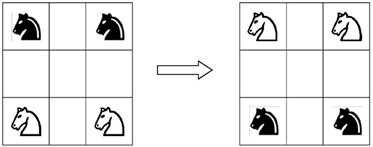
\includegraphics[keepaspectratio=true,scale=0.6]{HW1.jpg}}
\captionof{figure}{Start to Goal board state}    
\end{minipage}

\vspace{0.5cm}
\noindent The Four Knights puzzle is played on a 3 by 3 chess board. As depicted in \textit{Figure 1}, the opposing knights (two white and two black) begin in opposite corners. The goal of this puzzle is to have the opposing knights switch places on the three-by-three chess board. The knights are moved one at a time, using the standard movement rule (two squares ahead in any direction, then one square left or right), with alternating turns between black and white.  White will make the first move.

\noindent The puzzle will be expanded beyond a 3x3 to a 4x4 and a 5x5 board size.  There is also a scenario on the 5x5 board where the knights start in random positions, same goals and rules apply.
\newpage

\section{Algorithm Implementations}
\subsection{A* Implementation}
\noindent The python implementation of the A* search algorithm can be found in the linked repository above. The outline of how the A* algorithm is implemented is as follows:

\begin{verbatim}
    open_list is the list of states to be explored
    closed_list is the list of states that have been explored
    1. Input parameters: start_state, goal_state
    2. Add the start_state to the open_list.
    3. (Main loop) Keep looping while there is something in the open_list
    4. Grab the state in the open_list that has the lowest predicted cost
    5. Explore its children
    6. For each child do steps 7-9 
    7. If the child is the goal, return the path from start to goal.
    8. Since the child is not the goal, calculate its heuristic to the goal.
    9. If the the child is not in the open_list, 
       and the child is not in the closed_list, 
       add it to the open_list.
    10. Add the state that we just explored to the closed_list.
    11. Loop back to step 3.
    12. If no path has been found, return that no path was found.
\end{verbatim}

\newpage
\subsection{Branch and Bound Implementation}
The python implementation of the Branch and Bound search algorithm can be found in the linked repository above. The outline of how the Branch and Bound algorithm is implemented is as follows:

\begin{verbatim}
    open_list is the list of states to be explored
    closed_list is the list of states that have been explored
    1. Input parameters: start_state, goal_state
    2. Add the start_state to the open_list.
    3. (Main loop) Keep looping while there is something in the open_list
    4. Grab the state in the open_list that has the lowest cost.
       This effectively becomes backtracking once a new bound is set.
    5. Check if adding a child would be worse than the bound.
    6. If not then for each child do steps 7-8 
    7. If the child is the goal, set the bound to the path length.
    8. If the the child is not in the open_list,
       and its cost would be within the bound, 
       and the child is not in the closed_list, 
       add it to the open_list.
    9. Add the state that we just explored to the closed_list.
    10. Loop back to step 3.
    11. If we found a path return the path
    12. If no path has been found, return that no path was found.
\end{verbatim}
\newpage

\section{Heuristic Calculation}

\noindent The full implementation of the \texttt{calc\_heuristic()} function can be found in the linked repository above.

\noindent The heuristic equation for the A* algorithm where x is the manhattan distance between 2 points is as follows:

\vspace{0.5cm}

\begin{math}
\begin{array}{c} (x-1) \left((x-3) (x-2) \left(\left(\left(\left(\frac{x-7}{224}-\frac{5}{504}\right) (x-8)+\frac{149}{5040}\right) (x-5)-\frac{13}{120}\right) (x-4) x+\frac{2}{3}\right)-1\right)+3 \\ = \\ \frac{x^8}{224}-\frac{145 x^7}{1008}+\frac{227 x^6}{120}-\frac{9383 x^5}{720}+\frac{4811 x^4}{96}-\frac{7595 x^3}{72}+\frac{30517 x^2}{280}-\frac{8261 x}{210} \end{array}
\end{math}

\vspace{0.7cm}

\noindent This equation was selected via Lagrange Interpolation of given points.
\noindent The tool used to find this equation can be found here:

\url{https://www.dcode.fr/function-equation-finder}

\noindent For instance, if x = 0, the function will output 0. If x = 5 the function will output 2.
\noindent This is done to more optimally approximate the amount of moves that a knight would have to take to reach the goal.  This is due to the manner in which a knight moves.  Manhattan distance is not effecient enough for many scenarios. For example, having a Manhattan distance of 1 is not 1 step away from reaching that point but instead it is 3 steps.

\newpage

\section{Algorithm Analysis}
\subsection{A* Algorithm}
\noindent 3 separate data sets are created for this algorithm.  One is a heap and the other two are sets.  The heap is used for optimizing lookup of the next state to explore by ordering the heap according to its f score.  The sets are used for optimizing look ups of unique states.  The lookup associate with a heap is a pop method.  The pop method has a O(logn) due to the "sift-down" nature of heaps growing non-linearly.  Using sets allows for set look ups to be optimized down to O(1) due to hashing.  

\noindent Adding, or pushing, a state on to the heap has a O(logn) due to the "sift-up" nature of heaps growing non-linearly. Adding a state to a set has a O(1) due to hashing.

\noindent Furthermore, the algorithm itself can be analyzed as:

\begin{math}
n + n = 2n
\end{math}

\noindent Combine the algorithm analysis with the data set analysis to get:

\begin{math}
((2n) * (2logn + 1 + 1 + 1) = (2nlogn + 2n)
\end{math}

\noindent This function will be dominated by \begin{math} nlogn \end{math} therefore the time complexity of this A* algorithm is \begin{math} O(nlogn) \end{math}. This is fairly efficient.

\newpage
\subsection{Branch and Bound}
\noindent 3 separate data sets are created for this algorithm.  One is a heap and the other two are sets.  The heap is used for optimizing lookup of the next state to explore by ordering the heap according to its f score.  The sets are used for optimizing look ups of unique states.  The lookup associate with a heap is a pop method.  The pop method has a O(logn) due to the "sift-down" nature of heaps growing non-linearly.  Using sets allows for set look ups to be optimized down to O(1) due to hashing.  

\noindent Adding, or pushing, a state on to the heap has a O(logn) due to the "sift-up" nature of heaps growing non-linearly. Adding a state to a set has a O(1) due to hashing.

\noindent Furthermore, the algorithm itself can be analyzed as:

\begin{math}
n + (n-1) + (n-2 + (n-3) + ... + (n-(n-1)) = n(n + 1)/2 = (n^2 + n)/2
\end{math}

\noindent Combine the algorithm analysis with the data set analysis to get:

\begin{math}
((n^2 + n)/2) * (2logn + 1 + 1 + 1) = (n^2*2logn + n*2logn + 3n^2 + 3n)/2
\end{math}

\noindent This function will be dominated by \begin{math} n^2logn \end{math} therefore the time complexity of this Branch and Bound algorithm is \begin{math} O(n^2logn) \end{math}.  This is very inefficient.

\newpage

\subsection{Analysis Comparison and Recommendation}

\noindent The analysis of both algorithms shows that A* should out perform Branch and Bound in nearly every case.  In \textit{Figure 2} is the graphed comparison between the two time complexities.

\vspace{0.7cm}

\begin{minipage}{\linewidth} % to keep image and caption on one page
\makebox[\linewidth]{ %to center the image
  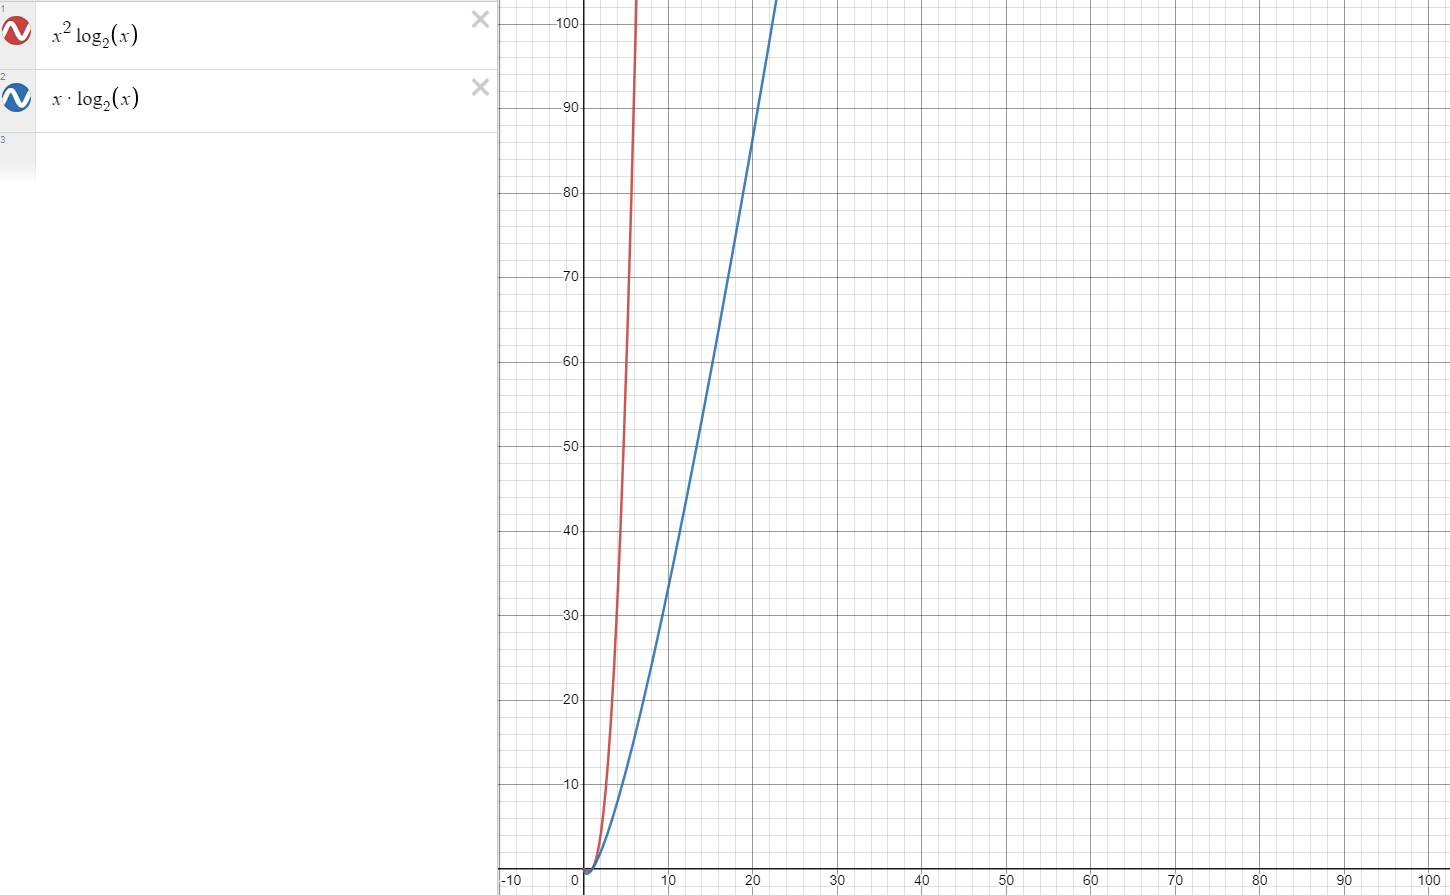
\includegraphics[keepaspectratio=true,scale=0.4]{Graphs.png}}
\captionof{figure}{A* and BnB BigO Comparison}    
\end{minipage}

\vspace{0.7cm}

\begin{center}
\begin{tabular}{|p{4cm}|p{4cm}|}
\hline
\textbf{A*} & \textbf{Branch and Bound} \\
\hline
\begin{math}O(nlogn)\end{math} & \begin{math}O(n^2logn)\end{math} \\
\hline
\end{tabular}
\end{center}


\noindent Due to the time complexities of both algorithms, as well as the rapid approach of A* to return the first path found rather than Branch and Bounds approach that always finds the optimal solution, I am going to recommend that A* be used for solving this problem and similar path-finding problems.

\newpage

\section{Metrics}

\noindent The 2 metrics that will be used to directly measure the efficiency of both algorithms will be the number of steps the algorithm took to reach the destination and the amount of time the algorithm took to run.

\noindent The number of steps will be the number of moves or state changes that the board makes until the goal is achieved.  This will be recorded and returned by the algorithm if the algorithm finds a solution.

\noindent The runtime will be the amount of time taken from immediately before the algorithm begins to run to immediately after the algorithm returns a value.

\newpage

\section{Design Considerations}

\noindent Both algorithms, their data structures, and their environments will be implemented in Python. This is not out of any particular optimizations to Python that make these algorithms, data structures, or environments more efficient, but out of ease of implementation.

\noindent The data structures implemented were selected due to optimizations in their behaviour.  Heaps and sets were implemented for their efficient lookup and management time complexities.

\noindent The custom data structures, \textit{Node} and \textit{ChessBoard}, were implemented for simple storage and traversal of necessary data.  The implementation of these data structures should have no impact on the time complexities of the rest of the program.

\newpage

\section{Test Plan}

\noindent To test the efficiency of both algorithms I will be implementing 3 hand-crafted test scenarios and 1 procedurally generated test scenario.  The 3 hand-crafted test scenarios are as follows:

\noindent A 3x3 chess board with the black knights starting in the upper 2 corners of the board and the white knights starting in the bottom 2 corners of the board.

\noindent A 4x4 chess board with the black knights starting in the upper 2 corners of the board and the white knights starting in the bottom 2 corners of the board.

\noindent A 5x5 chess board with the black knights starting in the upper 2 corners of the board and the white knights starting in the bottom 2 corners of the board.

\noindent The 1 procedurally generated test scenario is as follows:

\noindent A 5x5 chess board with the black and white knights starting in randomized positions.  The positions must be unique to all other previously selected positions.

\newpage

\section{Source Code}
\subsection{A* Algorithm}
\noindent The source code for the A* Algorithm can be found here: 

\url{https://github.com/DottsGit-UoMD-CIS-505/Final-Project/blob/master/src/a_star.py}

\subsection{Branch and Bound Algorithm}
\noindent The source code for the A* Algorithm can be found here: 

\url{https://github.com/DottsGit-UoMD-CIS-505/Final-Project/blob/master/src/branch_and_bound.py}

\newpage

\section{Test Case Compilation}
\subsection{Screen Prints}
\begin{minipage}{\linewidth} % to keep image and caption on one page
\makebox[\linewidth]{ %to center the image
  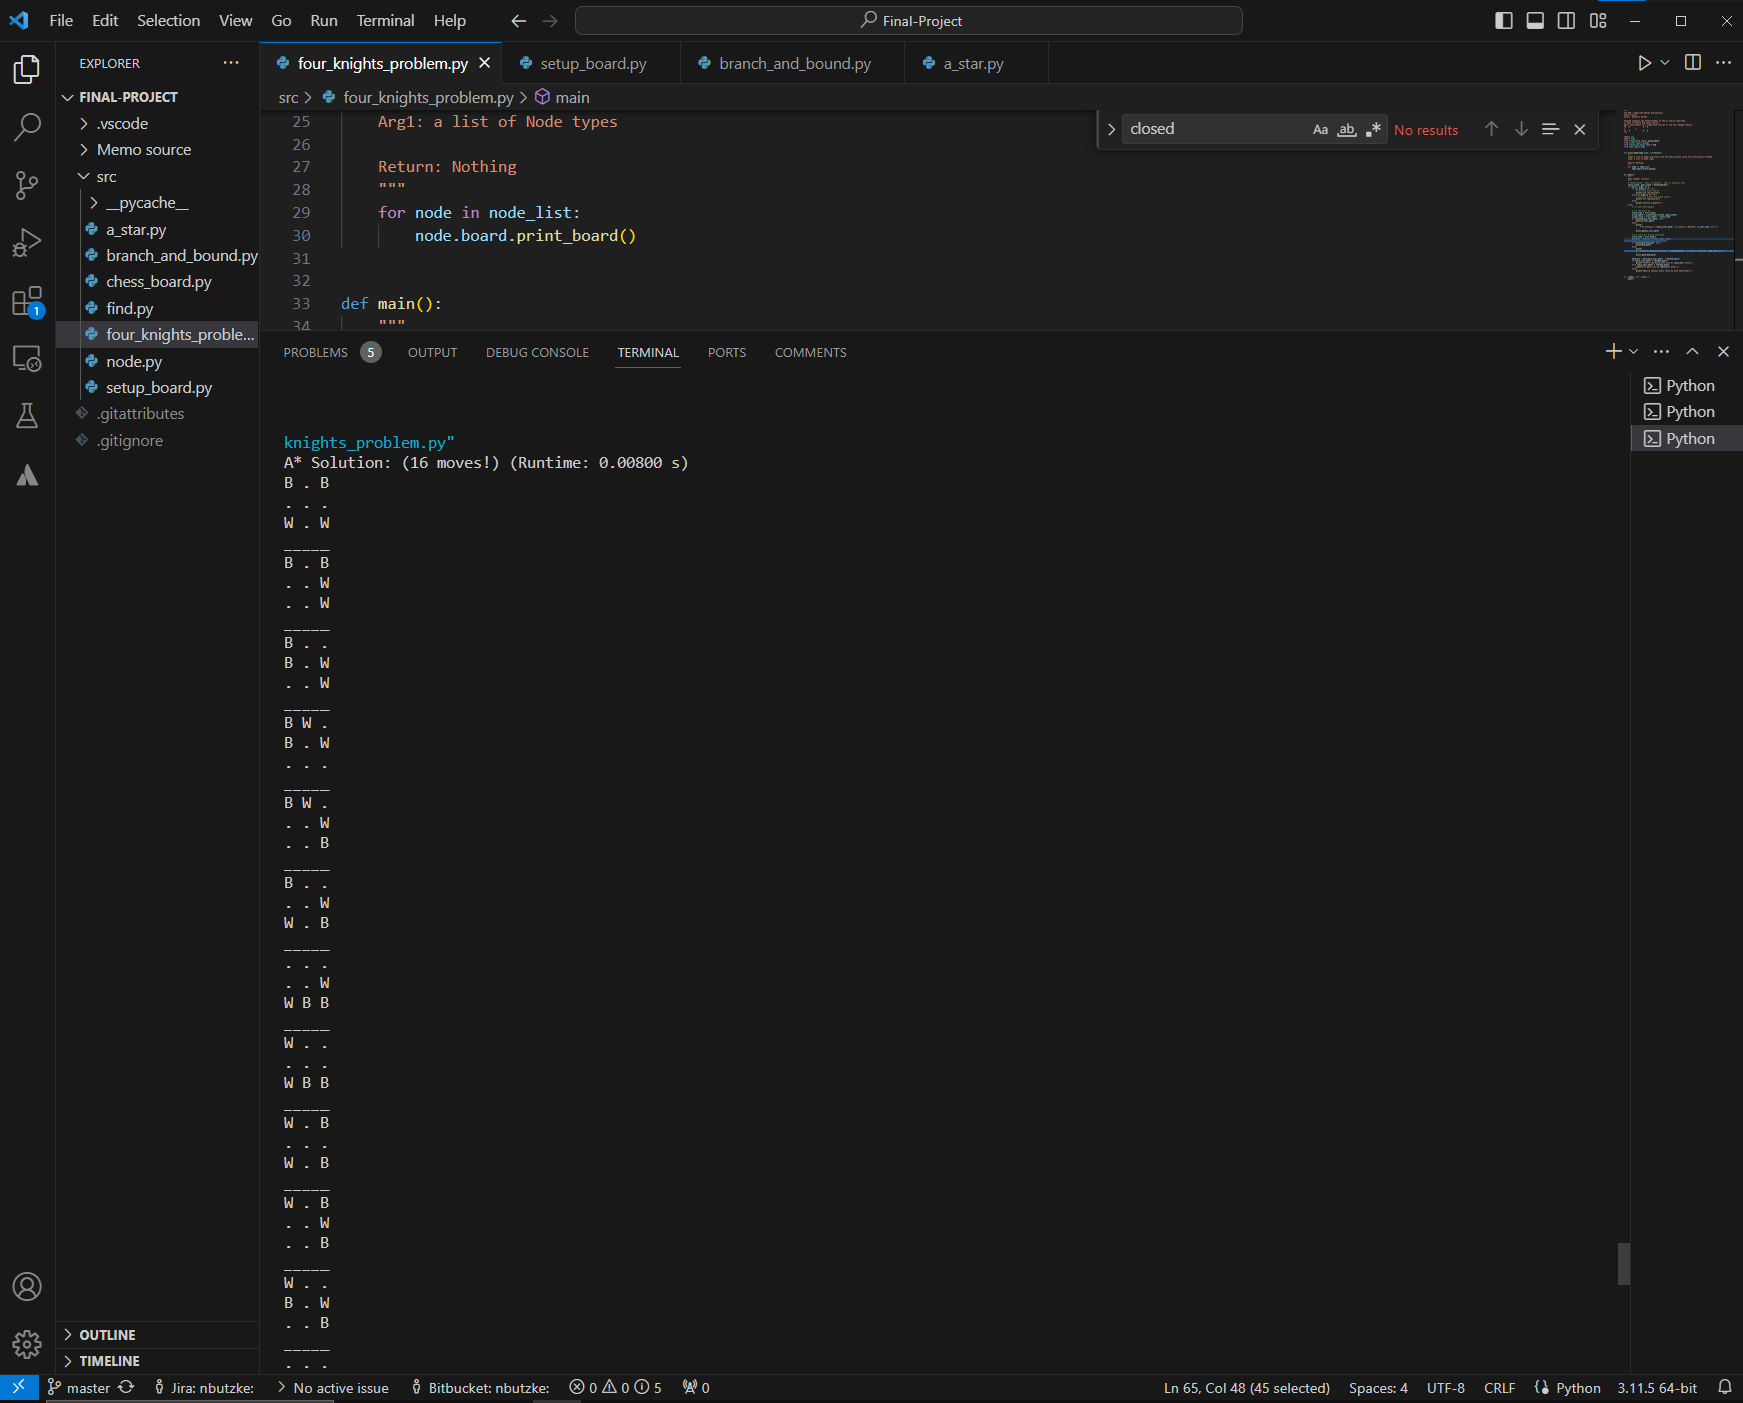
\includegraphics[keepaspectratio=true,scale=0.25]{A.png}}
\captionof{figure}{A* Screen Print}    
\end{minipage}
\begin{minipage}{\linewidth} % to keep image and caption on one page
\makebox[\linewidth]{ %to center the image
  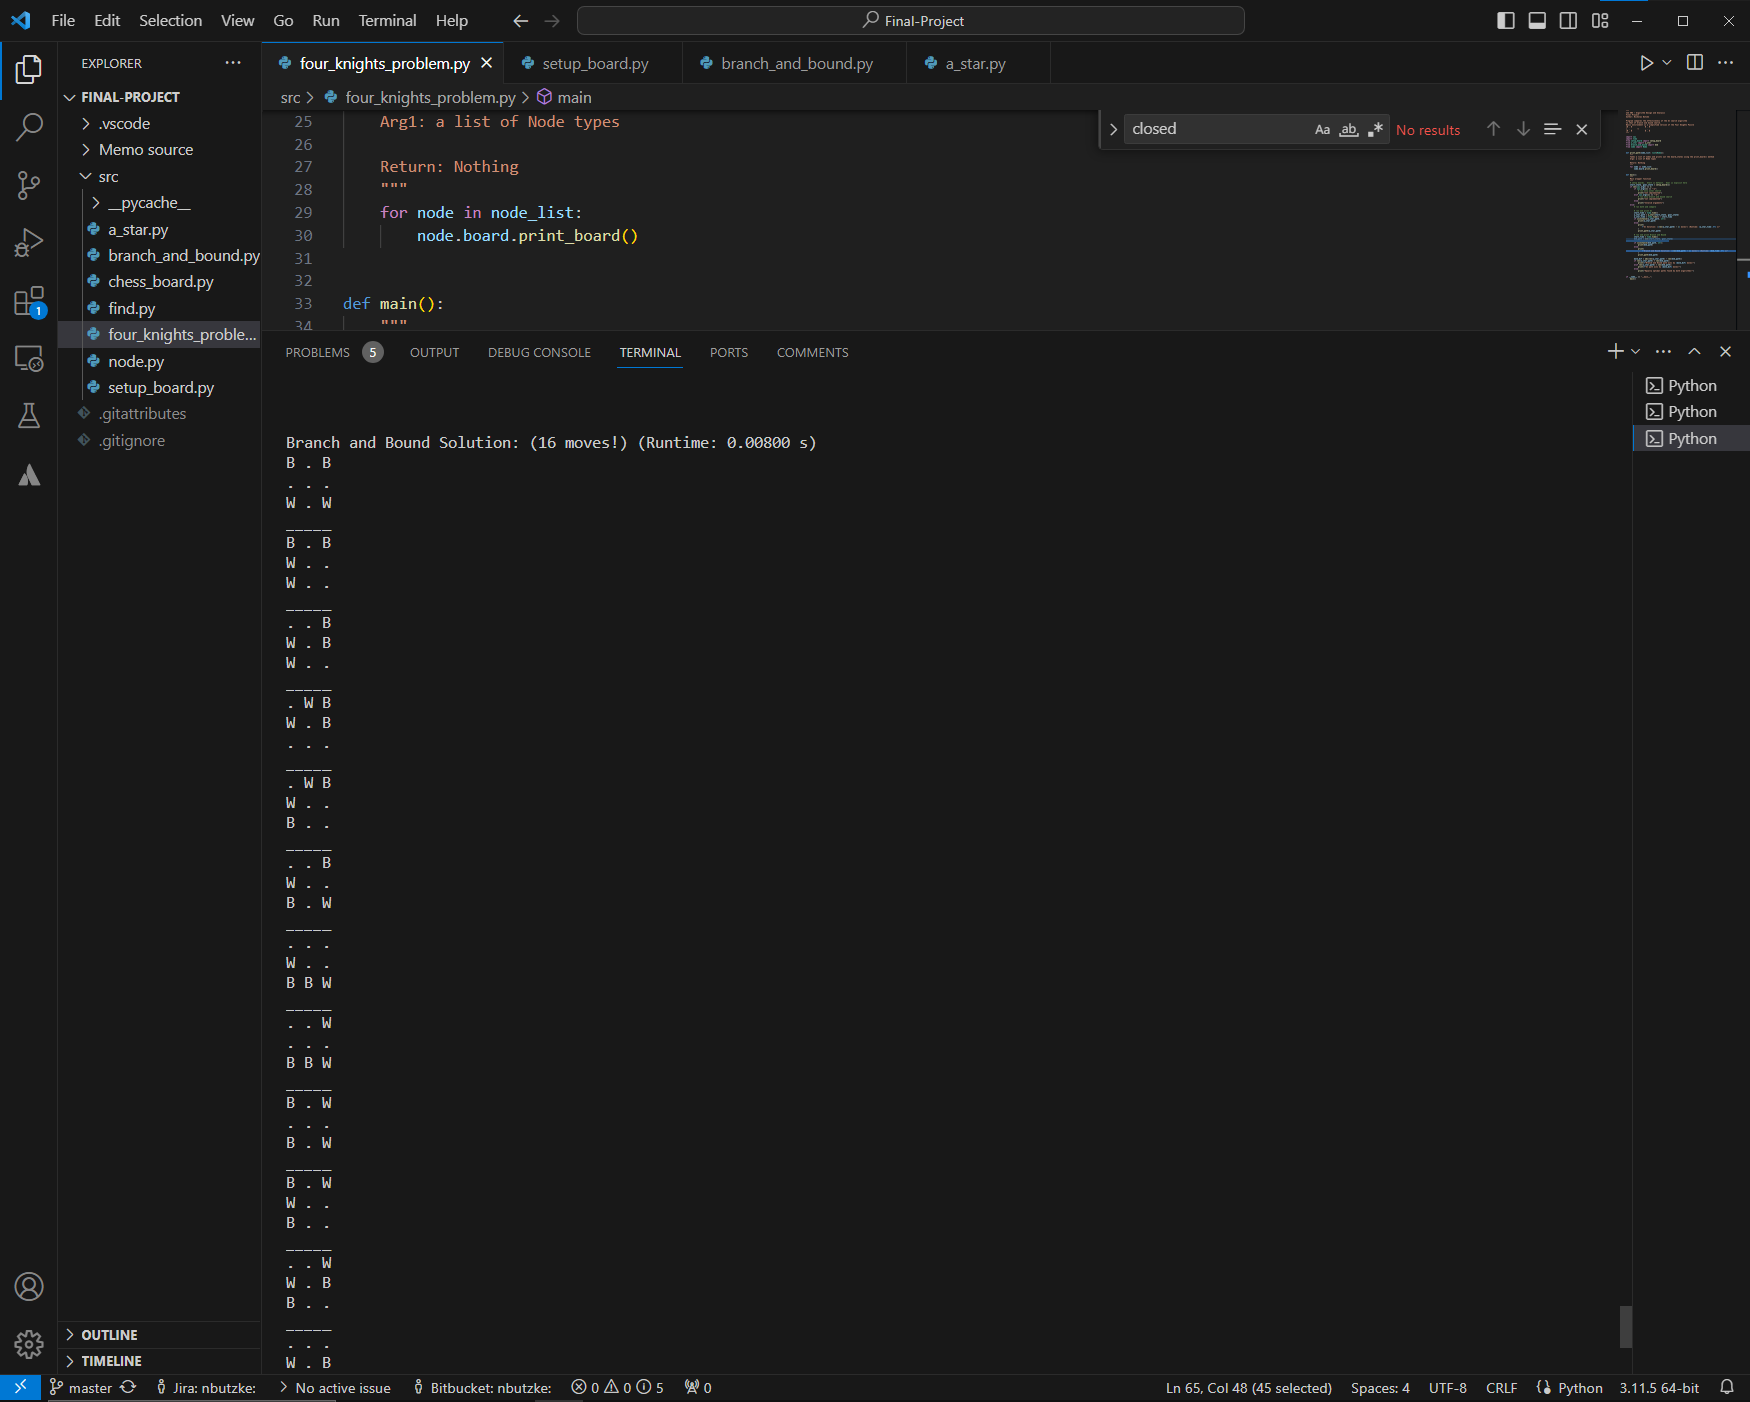
\includegraphics[keepaspectratio=true,scale=0.25]{B.png}}
\captionof{figure}{Branch and Bound Screen Print}    
\end{minipage}

\newpage

\subsection{Example Path Output}
\begin{multicols}{2}
\noindent A* search example path:

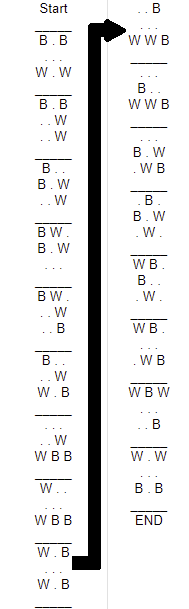
\includegraphics[scale=1]{AStarPath.png}
\vfill\null
\noindent Branch and Bound search example path:

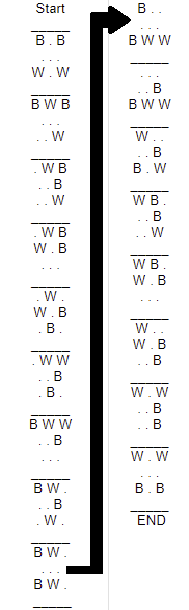
\includegraphics[scale=1]{bnbPath.png}
\end{multicols}
\newpage


\newpage

\section{Results and Results Analysis}
\subsection{3x3 Board (Hand-Crafted)}
Both algorithms found an optimal path of 16 moves.  Here are 10 runs performed on the 3x3 board:
\begin{center}
\begin{tabular}{|p{4cm}|p{4cm}|}
\hline
\textbf{A*} & \textbf{Branch and Bound} \\
\hline
8ms & 8ms \\
\hline
7ms & 7ms \\
\hline
8ms & 8ms \\
\hline
8ms & 8ms \\
\hline
7ms & 7ms \\
\hline
8ms & 8ms \\
\hline
8ms & 8ms \\
\hline
8ms & 7ms \\
\hline
8ms & 7ms \\
\hline
8ms & 7ms \\
\hline
\end{tabular}
\end{center}
\noindent The A* search algorithm ran for an average of 7.8ms over 10 runs.

\noindent The Branch and Bound Algorithm ran for an average of 7.5ms over 10 runs.

\noindent A* and Branch and found equally optimal solutions in practically the same amount of time.  The 0.3ms difference is within margin of error and is therefore non-significant.  In this case, and according to the results, the original recommendation favoring A* over Branch and Bound was correct.

\newpage

\subsection{4x4 Board (Hand-Crafted)}
Both algorithms found an optimal path of 8 moves.  Here are 10 runs performed on the 4x4 board:
\begin{center}
\begin{tabular}{|p{4cm}|p{4cm}|}
\hline
\textbf{A*} & \textbf{Branch and Bound} \\
\hline
8ms & 216ms \\
\hline
8ms & 215ms \\
\hline
7ms & 211ms \\
\hline
7ms & 212ms \\
\hline
8ms & 207ms \\
\hline
8ms & 218ms \\
\hline
8ms & 211ms \\
\hline
8ms & 205ms \\
\hline
8ms & 210ms \\
\hline
9ms & 212ms \\
\hline
\end{tabular}
\end{center}
\noindent The A* search algorithm ran for an average of 7.9ms over 10 runs.

\noindent The Branch and Bound Algorithm ran for an average of 211.7ms over 10 runs.

\noindent A* and Branch and found equally optimal solutions significantly different amounts of time.  On average, it took Branch and Bound 2,680\% longer than A* to find a solution. In this case, and according to the results, the original recommendation favoring A* over Branch and Bound was correct.

\newpage

\subsection{5x5 Board (Hand-Crafted)}
Both algorithms found an optimal path of 12 moves.  Here are 10 runs performed on the 5x5 board:
\begin{center}
\begin{tabular}{|p{4cm}|p{4cm}|}
\hline
\textbf{A*} & \textbf{Branch and Bound} \\
\hline
23ms & 7,005ms \\
\hline
23ms & 7,006ms \\
\hline
24ms & 7,398ms \\
\hline
23ms & 7,056ms \\
\hline
24ms & 7,018ms \\
\hline
24ms & 6,998ms \\
\hline
30ms & 7,151ms \\
\hline
24ms & 7,039ms \\
\hline
24ms & 7,039ms \\
\hline
23ms & 7,034ms \\
\hline
\end{tabular}
\end{center}
\noindent The A* search algorithm ran for an average of 24.2ms over 10 runs.

\noindent The Branch and Bound Algorithm ran for an average of 7,074.4ms over 10 runs.

\noindent A* and Branch and found equally optimal solutions in vastly different amounts of time.  On average, it took Branch and Bound 29,233\% longer than A* to find a solution. In this case, and according to the results, the original recommendation favoring A* over Branch and Bound was correct.

\newpage

\subsection{5x5 Board (Procedurally Generated)}
Both algorithms found an optimal path each time. The moves are displayed in the 3rd column.  Here are 10 runs performed on the procedurally generated 5x5 board:
\begin{center}
\begin{tabular}{|p{4cm}|p{4cm}|p{4cm}|}
\hline
\textbf{A*} & \textbf{Branch and Bound} & \textbf{Move Count} \\
\hline
2050ms & 10,807ms & 14 \\
\hline
38ms & 1,999ms & 8 \\
\hline
336ms & 9,475ms & 12 \\
\hline
65ms & 6,783ms & 10 \\
\hline
160ms & 8,132ms & 10 \\
\hline
30ms & 2,720ms & 8 \\
\hline
255ms & 7,250ms & 10 \\
\hline
14ms & 1,991ms & 8 \\
\hline
57ms & 6,052ms & 10 \\
\hline
34ms & 3,294ms & 8\\
\hline
\end{tabular}
\end{center}
\noindent The A* search algorithm ran for an average of 303.9ms over 10 runs.

\noindent The Branch and Bound Algorithm ran for an average of 5,850.3ms over 10 runs.

\noindent A* and Branch and found equally optimal solutions in every scenario however it was in vastly different amounts of time.  On average, it took Branch and Bound 1,925\% longer than A* to find a solution. In this case, and according to the results, the original recommendation favoring A* over Branch and Bound was correct.

\newpage

\section{Conclusion}
While the A* search algorithm and the Branch and Bound search algorithm both found equally optimal paths from the initial state to the goal state in every scenario, A* search completed the task in significantly less amount of time.  Even when more difficult or novel scenarios were presented, A* search consistently out performed Branch and Bound.  This is consistent with the hypothesis, algorithm analysis comparison, and algorithm recommendations.  Unless a specific scenario is presented that would favor Branch and Bound, use A*.

\end{document}